%\begin{frame}[label=intro1]{Einführungsaufgabe 1}
%    Der Geheimtext lautet:
%    \begin{center}
%        AMEHT SEGITHCIW NIE TSI EIGOLOTPYRK
%    \end{center}
%    Stellen Sie den ursprünglichen Text wieder her.
%\end{frame}
%
%\begin{frame}[label=intro1Sol]{Lösung der Einführungsaufgabe 1}
%    \begin{center}
%    
%        Geheimtext:\\
%        AMEHT SEGITHCIW NIE TSI EIGOLOTPYRK\\
%        \bigskip
%        ursprünglicher Text:\\
%        KRYPTOLOGIE IST EIN WICHTIGES THEMA\\
%    \end{center}
%    Der Geheimtext entspricht dem von rechts nach links (rückwärts) gelesenen ursprünglichen Text.
%\end{frame}
%
%\begin{frame}[label=intro2]{Einführungsaufgabe 2}
%    Der Geheimtext lautet:
%    \begin{center}
%    \small
%        \begin{enumerate}
%            \item RKPYOTOLIGEEMREOLGCITHEGEHMIINSSE
%            \item HCSFIRILTAHCZFUEBUHAWNERDNUKUZMMOINUEIZNER
%        \end{enumerate}
%        \normalsize
%    \end{center}
%    Stellen Sie den ursprünglichen Text wieder her.
%\end{frame}
%
%\begin{frame}[label=intro2Sol]{Lösung Einführungsaufgabe 2}
%    Geheimtext:
%    \begin{center}
%    \small
%        \begin{enumerate}
%            \item RKPYOTOLIGEEMREOLGCITHEGEHMIINSSE
%            \item HCSFIRILTAHCZFUEBUHAWNERDNUKUZMMOINUEIZNER
%        \end{enumerate}
%        \normalsize
%    \end{center}
%    Ursprünglicher Text:
%    \begin{center}
%    \small
%        \begin{enumerate}
%            \item KRYPTOLOGIE ERMOEGLICHT GEHEIMNISSE
%            \item SCHRIFTLICH AUFZUBEWAHREN UND ZU KOMMUNIZIEREN
%        \end{enumerate}
%        \normalsize
%    \end{center}
%    Der Geheimtext entsteht durch Austauschen der Positionen der Buchstaben.
%    \begin{figure}[H]
%        \centering
%        \begin{subfigure}[b]{0.45\textwidth}
%          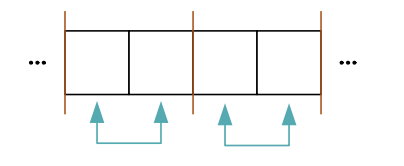
\includegraphics[width=\textwidth]{GrundlagenInfo/03_Kryptologie/Figures/krypto_swap_2.png}\caption{\enquote{Zweiertausch}}
%        \end{subfigure}
%        \hfill
%        \begin{subfigure}[b]{0.45\textwidth}
%          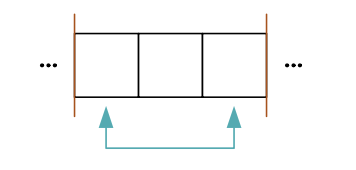
\includegraphics[width=\textwidth]{GrundlagenInfo/03_Kryptologie/Figures/krypto_swap_3.png}\caption{\enquote{Dreiertausch}}
%        \end{subfigure}
%    \end{figure}
%\end{frame}
%
%\begin{frame}[fragile, label=sol22]{\enquote{Zweiertausch} in Python \emoji{snake}}
%\begin{lstlisting}
%def zweiertausch(klartext):
%    geheimtext = "" # leerer String
%    b = 0
%    while b < (len(klartext) - 1):
%        geheimtext += klartext[b + 1] + klartext[b]
%        b += 2
%
%    if len(klartext) % 2 != 0:
%        # Klartexte ungerader Länge
%        geheimtext += klartext[len(klartext) - 1]
%    print(geheimtext)
%
%
%zweiertausch("KANTONSSCHULE")
%\end{lstlisting}
%\end{frame}
%
%\begin{frame}[label=python2]{\enquote{Dreiertausch} in Python \emoji{snake}}
%\abgabebox{Skript, Aufgabe 2.5}
%\end{frame}

